\documentclass{article}%
\usepackage[T1]{fontenc}%
\usepackage[utf8]{inputenc}%
\usepackage{lmodern}%
\usepackage{textcomp}%
\usepackage{lastpage}%
\usepackage[head=40pt,margin=0.5in,bottom=0.6in]{geometry}%
\usepackage{graphicx}%
%
\title{\textbf{Trabajadores “revolucionarios” protestaron en Ciudad Guayana}}%
\author{El Nacional Web}%
\date{09/10/2018}%
%
\begin{document}%
\normalsize%
\maketitle%
\textbf{URL: }%
http://www.el{-}nacional.com/noticias/protestas/trabajadores{-}revolucionarios{-}protestan{-}ciudad{-}guayana\_254985\newline%
%
\textbf{Periodico: }%
EN, %
ID: %
254985, %
Seccion: %
Protestas\newline%
%
\textbf{Palabras Claves: }%
Economía, Crisis económica, Protestas, Denuncia, Bolívar\newline%
%
\textbf{Derecho: }%
2.3, %
Otros Derechos: %
2.1, %
Sub Derechos: %
2.3.4, 2.1.1\newline%
%
\textbf{EP: }%
SI\newline%
\newline%
%
\textbf{\textit{Los empleados de las empresas básicas rechazaron la eliminación de tablas salariales y del seguro HCM}}%
\newline%
\newline%
%
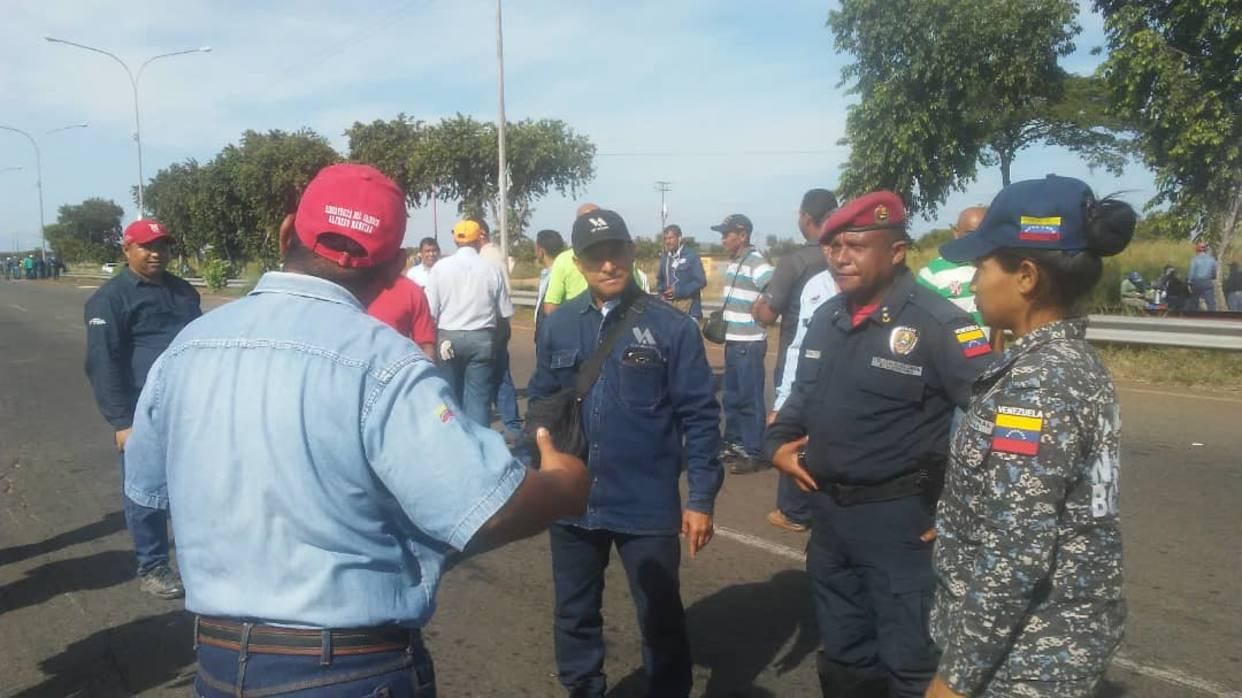
\includegraphics[width=300px]{10.jpg}%
\newline%
%
La mañana de este martes los trabajadores de las empresas básicas de Ciudad Guayana, ubicada en el estado Bolívar, protestaron en contra de la eliminación de tablas salariales.%
\newline%
%
Los manifestantes trancaron el paso de los peajes de la ciudad para evitar que los vehículos ingresen o salgan de la misma.%
\newline%
%
Un manifestante denunció ante la Guardia Nacional Bolivariana que eliminaron el seguro HCM que cubre los gastos médicos de los empleados y declaró que los trabajadores de las empresas básicas también son revolucionarios.%
\newline%
%
“Nosotros en 2014 fuimos los que quitamos las guarimbas”, recordó.%
\newline%
%
Usuarios de Twitter rechazaron las protestas de los trabajadores de las empresas básicas porque recuerdan que los mismos no han sido parte de las manifestaciones de otros gremios y que solo velan por sus intereses.%
\newline%
%
\end{document}